\documentclass[12pt,a4paper]{article}

% ── Packages ──────────────────────────────────────────────────────────────────
\usepackage[T1]{fontenc}
\usepackage[english]{babel}
\usepackage{geometry}
\usepackage{amsmath,amssymb,amsthm}
\usepackage{mathtools}
\usepackage{algorithm}
\usepackage{algpseudocode}
\usepackage{booktabs}
\usepackage{array}
\usepackage{tabularx}
\usepackage{multirow}
\usepackage{graphicx}
\usepackage{float}
\usepackage{xcolor}
\usepackage{listings}
\usepackage{enumitem}
\usepackage{caption}
\usepackage{subcaption}
\usepackage{hyperref}
\usepackage{cleveref}
\usepackage{tikz}
\usepackage{pgfplots}
\pgfplotsset{compat=1.18}
\usetikzlibrary{shapes.geometric, arrows.meta, positioning, calc, patterns}

\geometry{
  a4paper,
  top=25mm, bottom=25mm,
  left=25mm, right=25mm
}

\hypersetup{
  colorlinks=true,
  linkcolor=blue!60!black,
  citecolor=blue!60!black,
  urlcolor=blue!60!black
}

% ── Code listing style ────────────────────────────────────────────────────────
\lstdefinestyle{sqlstyle}{
  language=SQL,
  basicstyle=\ttfamily\small,
  keywordstyle=\bfseries\color{blue!70!black},
  commentstyle=\itshape\color{gray},
  stringstyle=\color{green!50!black},
  breaklines=true,
  frame=single,
  numbers=left,
  numberstyle=\tiny\color{gray},
  xleftmargin=1.5em
}

% ── Theorem environments ──────────────────────────────────────────────────────
\theoremstyle{definition}
\newtheorem{definition}{Definition}[section]
\newtheorem{property}{Property}[section]
\theoremstyle{plain}
\newtheorem{theorem}{Theorem}[section]
\newtheorem{lemma}[theorem]{Lemma}
\theoremstyle{remark}
\newtheorem{remark}{Remark}[section]

% ── Custom commands ───────────────────────────────────────────────────────────
\newcommand{\R}{\mathbb{R}}
\newcommand{\N}{\mathbb{N}}
\newcommand{\Z}{\mathbb{Z}}
\newcommand{\norm}[1]{\left\lVert #1 \right\rVert}
\newcommand{\abs}[1]{\left\lvert #1 \right\rvert}
\newcommand{\vect}[1]{\mathbf{#1}}
\newcommand{\coord}[2]{(#1,\,#2)}
\newcommand{\HMAC}{\operatorname{HMAC}}
\newcommand{\SHA}{\operatorname{SHA\text{-}256}}
\newcommand{\bcrypt}{\operatorname{bcrypt}}
\DeclareMathOperator{\rad}{rad}
\DeclareMathOperator{\sgn}{sgn}
\DeclareMathOperator{\dist}{dist}
\DeclareMathOperator{\proj}{proj}
\DeclareMathOperator*{\argmin}{arg\,min}

% ── Title block ───────────────────────────────────────────────────────────────
\title{%
  \textbf{NARS: Mathematical Foundations of a National Addressing Reference System}\\[4pt]
  \large Geometric Validation, Spatial Algorithms, and Security Primitives
  for a Multi-Layer Urban Feature Database
}

\author{%
  \textbf{Software Engineering Report} \\[4pt]
  National Addressing Reference System (NARS) v2.0 \\
  ASP.NET Core 10 / Vue 3 / PostGIS
}

\date{\today}

% ══════════════════════════════════════════════════════════════════════════════
\begin{document}
\maketitle
\tableofcontents
\newpage

% ══════════════════════════════════════════════════════════════════════════════
\begin{abstract}
The National Addressing Reference System (NARS) is a full-stack geospatial
application designed for the systematic capture and validation of urban
addressing features across Algerian administrative divisions (Wilayas,
Daïras, and Communes). This document formalises the mathematical and
algorithmic foundations that underpin eight distinct feature types: urban
areas, districts, city centres, roads, house entrances, public buildings,
public spaces, and naming panels.

We derive the geodetic distance metrics (Haversine formula), the angular
deviation predicates used in road validation, the polygon adjacency and
coverage conditions governing district layout, the pixel-space snap
geometry used during interactive drawing, and the scattered-area
auto-computation pipeline. On the security side, we present the HMAC-SHA256
JWT construction, the BCrypt password hashing scheme, the SHA-256 refresh
token storage protocol, the sliding-window rate-limiting model, and the
antiforgery token mechanism.

All equations are derived directly from the production source code; no
approximation or simplification has been introduced. The document is
intended to serve as both a correctness reference and a foundation for
formal verification of the validation rules embedded in the system.
\end{abstract}

\noindent\textbf{Keywords:} geographic information systems, spatial validation,
geodesy, JWT authentication, polygon coverage, snap geometry, PostGIS,
algorithmic correctness

% ══════════════════════════════════════════════════════════════════════════════
\section{Introduction}
\label{sec:intro}

Urban addressing is a prerequisite for emergency response, postal delivery,
property registration, and infrastructure planning. In Algeria, addresses are
structured hierarchically: a Wilaya (province) contains Daïras (districts),
each of which contains Communes (municipalities). NARS provides an
authenticated, multi-tenant web application that allows commune-level
operators to digitise and validate the spatial features that constitute an
address.

The system enforces a strict geometric ordering on feature creation.
\Cref{fig:feature_hierarchy} shows the dependency graph; a feature of
type $B$ may only be created after all prerequisites of type $A$ exist and
pass their validation predicates. This ordering is not merely a UX
constraint --- it encodes spatial invariants that the system must maintain
in the PostGIS database.

\begin{figure}[H]
\centering
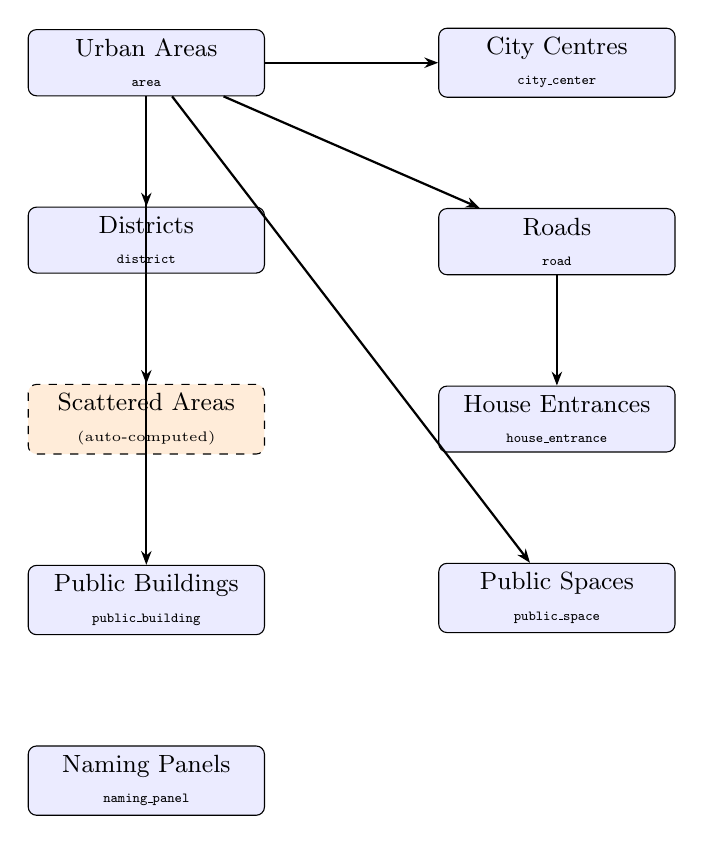
\begin{tikzpicture}[
  node distance=1.4cm and 2.2cm,
  box/.style={draw, rounded corners=3pt, minimum width=3cm,
              minimum height=0.8cm, align=center,
              fill=blue!8, font=\small},
  auto/.style={draw, rounded corners=3pt, minimum width=3cm,
               minimum height=0.8cm, align=center,
               fill=orange!15, font=\small, dashed},
  arr/.style={-{Stealth[length=5pt]}, thick}
]
\node[box] (area)    {Urban Areas\\{\tiny \texttt{area}}};
\node[box, right=of area] (cc) {City Centres\\{\tiny \texttt{city\_center}}};
\node[box, below=of area] (dist) {Districts\\{\tiny \texttt{district}}};
\node[box, below=of cc]   (road) {Roads\\{\tiny \texttt{road}}};
\node[auto, below=of dist] (scat) {Scattered Areas\\{\tiny (auto-computed)}};
\node[box, below=of road]  (he)   {House Entrances\\{\tiny \texttt{house\_entrance}}};
\node[box, below=of scat]  (pb)   {Public Buildings\\{\tiny \texttt{public\_building}}};
\node[box, below=of he]    (ps)   {Public Spaces\\{\tiny \texttt{public\_space}}};
\node[box, below=of pb]    (np)   {Naming Panels\\{\tiny \texttt{naming\_panel}}};

\draw[arr] (area) -- (dist);
\draw[arr] (area) -- (cc);
\draw[arr] (area) -- (road);
\draw[arr] (dist) -- (scat);
\draw[arr] (road) -- (he);
\draw[arr] (area) -- (pb);
\draw[arr] (area) -- (ps);
\end{tikzpicture}
\caption{Feature dependency graph. Dashed nodes are auto-computed by the
background task queue; solid nodes require explicit operator input.}
\label{fig:feature_hierarchy}
\end{figure}

The remainder of this document is organised as follows.
\Cref{sec:geodesy} establishes the geodetic coordinate model.
\Cref{sec:feature_types} describes the eight feature types and their
invariants. \Cref{sec:validation} derives all validation predicates in
closed form. \Cref{sec:snap} formalises the snap-geometry algorithm used
during interactive drawing. \Cref{sec:scattered} describes the
scattered-area computation. \Cref{sec:security} covers the authentication
and authorisation primitives. \Cref{sec:ratelimit} presents the
rate-limiting model. \Cref{sec:api} summarises the REST API surface.
\Cref{sec:conclusions} offers concluding remarks.

% ══════════════════════════════════════════════════════════════════════════════
\section{Geodetic Coordinate Model}
\label{sec:geodesy}

\subsection{Reference Ellipsoid and Projection}

All coordinates in NARS are stored and transmitted in geographic
coordinates (longitude $\lambda$, latitude $\varphi$) referenced to the
World Geodetic System 1984 (WGS84), corresponding to EPSG:4326. PostGIS
geometry columns use SRID 4326; geography columns use the same datum and
enable spheroidal distance computations.

\begin{definition}[Geographic coordinate]
A geographic coordinate is an ordered pair $p = \coord{\lambda}{\varphi}$
where $\lambda \in [-180^\circ, 180^\circ]$ is the longitude and
$\varphi \in [-90^\circ, 90^\circ]$ is the latitude.
\end{definition}

\subsection{Haversine Distance}

Client-side distance computations (circle radius estimation, road length
checks) use the Haversine formula. Given two geographic coordinates
$p_1 = \coord{\lambda_1}{\varphi_1}$ and $p_2 = \coord{\lambda_2}{\varphi_2}$,
the great-circle distance is:

\begin{equation}
  d(p_1, p_2) = 2 R \arctan\!\left(\frac{\sqrt{a}}{\sqrt{1 - a}}\right)
  \label{eq:haversine}
\end{equation}

where
\begin{equation}
  a = \sin^2\!\left(\frac{\Delta\varphi}{2}\right)
    + \cos\varphi_1 \cdot \cos\varphi_2 \cdot \sin^2\!\left(\frac{\Delta\lambda}{2}\right)
  \label{eq:haversine_a}
\end{equation}

with $\Delta\varphi = \varphi_2 - \varphi_1$ and
$\Delta\lambda = \lambda_2 - \lambda_1$ in radians, and the mean Earth
radius $R = 6{,}371{,}000\ \mathrm{m}$ (the value used throughout the
codebase; see \texttt{GEOMETRY\_CONFIG.\allowbreak earthRadiusMeters} in
\texttt{src/config.ts}).

\begin{remark}
The Haversine formula is numerically stable for all distances, including
antipodal points, unlike the simpler spherical law of cosines. PostGIS
server-side geography distances use the WGS84 spheroid, which introduces
a relative error below $0.3\,\%$ compared to Haversine; this discrepancy
is acceptable for all NARS use cases.
\end{remark}

\subsection{Circle Approximation}

City centres are stored as (centre, radius) pairs and rendered as
$n$-sided regular polygons. The $k$-th vertex of the approximating polygon is:

\begin{equation}
  v_k = \left(
    \lambda_c + \frac{r}{R\cos\varphi_c} \cdot \cos\!\left(\frac{2\pi k}{n}\right),\;
    \varphi_c + \frac{r}{R} \cdot \sin\!\left(\frac{2\pi k}{n}\right)
  \right), \quad k = 0, \ldots, n-1
  \label{eq:circle_vertex}
\end{equation}

where $\coord{\lambda_c}{\varphi_c}$ is the centre, $r$ the radius in
metres, and $n$ the number of segments. Two values are used:
$n = 64$ for rendering (smooth appearance) and $n = 16$ for edit mode
(lighter vertex handle count).

\subsection{Coordinate Encoding}

Features are persisted as JSON objects in a PostgreSQL \texttt{text} column.
The coordinates array uses the convention $\{$\texttt{lat}, \texttt{lng}$\}$
(latitude-first), while GeoJSON and PostGIS use longitude-first
$[\lambda, \varphi]$. All SQL fragments in \texttt{SqlFragments.cs} perform
the swap explicitly:

\begin{lstlisting}[style=sqlstyle, caption={Coordinate-order swap in SQL fragment}]
json_build_array(
    (c->>'lng')::float,   -- longitude first (GeoJSON)
    (c->>'lat')::float    -- latitude second
)
\end{lstlisting}

% ══════════════════════════════════════════════════════════════════════════════
\section{Feature Type Taxonomy}
\label{sec:feature_types}

\subsection{Type and Layer Hierarchy}

Each persisted feature carries two discriminators: a \emph{type} (one of
eight top-level classes) and a \emph{layer} (a subtype within that class).
\Cref{tab:feature_types} enumerates the full taxonomy.

\begin{table}[H]
\centering
\caption{Feature type and layer taxonomy}
\label{tab:feature_types}
\begin{tabularx}{\textwidth}{llXl}
\toprule
\textbf{Type key} & \textbf{Table} & \textbf{Layer keys} & \textbf{Geometry} \\
\midrule
\texttt{area} & \texttt{areas} &
  \texttt{central\_urban}, \texttt{secondary\_urban}, \texttt{scattered}$^*$
  & Polygon \\
\texttt{district} & \texttt{districts} &
  \texttt{housing\_estate}, \texttt{urban\_pole}, \texttt{district},
  \texttt{trad\_activities\_zone}, \texttt{industry\_zone}
  & Polygon \\
\texttt{city\_center} & \texttt{city\_centers} &
  \texttt{city\_center} & Point + radius \\
\texttt{road} & \texttt{roads} &
  \texttt{boulevard}, \texttt{avenue}, \texttt{street}, \texttt{drive},
  \texttt{lane}, \texttt{cul\_de\_sac}, \texttt{way}
  & LineString \\
\texttt{house\_entrance} & \texttt{house\_entrances} &
  \texttt{main\_entrance}, \texttt{secondary\_entrance} & Point \\
\texttt{public\_building} & \texttt{public\_buildings} &
  \texttt{public\_building} & Point \\
\texttt{public\_space} & \texttt{public\_spaces} &
  \texttt{garden}, \texttt{square} & Polygon \\
\texttt{naming\_panel} & \texttt{naming\_panels} &
  \texttt{naming\_panel} & Point \\
\bottomrule
\multicolumn{4}{l}{$^*$Auto-computed; cannot be saved manually.}
\end{tabularx}
\end{table}

\subsection{Feature Registry}

A central \texttt{feature\_registry} table maintains a
(UUID, type-string) index over all eight type tables, enabling
$O(1)$ type lookup given only a feature ID. The invariant is:

\begin{equation}
  \forall\, r \in \texttt{feature\_registry}: r.\mathit{id} \in
  \bigcup_{T \in \mathcal{T}} \pi_{\mathit{id}}(T)
  \label{eq:registry_invariant}
\end{equation}

where $\mathcal{T}$ is the set of eight type tables and $\pi_{\mathit{id}}$
denotes projection onto the ID column. This invariant is enforced by the
transactional insert in \texttt{SaveFeature} and by the dynamic
orphan-cleanup query in \texttt{ClearFeatures}.

\subsection{Payload Bounds}

To guard against memory exhaustion, two numeric bounds are enforced
server-side:

\begin{align}
  \abs{\texttt{rawJson}} &\leq C_{\text{payload}} = 524{,}288\ \text{bytes} \quad
  (= 512\ \text{KiB})
  \label{eq:payload_bound} \\
  \abs{\mathcal{C}} &\leq C_{\text{coords}} = 10{,}000
  \label{eq:coord_bound}
\end{align}

where $\abs{\mathcal{C}}$ is the cardinality of the coordinate array in a
validation request. In addition, all coordinate values are checked for
membership in $\R \setminus (\{\mathrm{NaN}\} \cup \{+\infty, -\infty\})$
before any PostGIS query is executed.

% ══════════════════════════════════════════════════════════════════════════════
\section{Geometric Validation Predicates}
\label{sec:validation}

\subsection{Road Validation}
\label{sec:road_validation}

A road is defined as an ordered sequence of geographic coordinates
$\mathcal{R} = (p_0, p_1, \ldots, p_{m-1})$ with $m \geq 2$.
Two predicates must hold before a road is accepted.

\subsubsection{Angular Deviation Bound}

For any three consecutive vertices $A = p_i$, $B = p_{i+1}$, $C = p_{i+2}$
define the planar direction vectors (in the longitude--latitude plane):

\begin{align}
  \vect{u} &= \coord{\lambda_B - \lambda_A}{\varphi_B - \varphi_A} \\
  \vect{v} &= \coord{\lambda_C - \lambda_B}{\varphi_C - \varphi_B}
\end{align}

The deflection angle $\theta_i$ at vertex $B$ is:

\begin{equation}
  \theta_i = \arccos\!\left(
    \frac{\vect{u} \cdot \vect{v}}{\norm{\vect{u}}_2 \cdot \norm{\vect{v}}_2}
  \right), \quad
  \theta_i \in [0^\circ, 180^\circ]
  \label{eq:road_angle}
\end{equation}

The road is valid if and only if:

\begin{equation}
  \forall\, i \in \{0, \ldots, m-3\}:
  \theta_i \leq \Theta_{\max} = 90^\circ
  \label{eq:road_angle_predicate}
\end{equation}

\begin{remark}
The dot product is clamped to $[-1, 1]$ before the $\arccos$ to prevent
floating-point errors from producing a domain exception. The check is
skipped when $\norm{\vect{u}}_2 < 10^{-10}$ or $\norm{\vect{v}}_2 < 10^{-10}$
(coincident vertices), which is correct as degenerate segments carry no
directional information.
\end{remark}

\subsubsection{Network Connectivity}

A new road $R_{\text{new}}$ must spatially connect to the existing road
network $\mathcal{N}$ (unless $\mathcal{N} = \emptyset$, i.e.\ this is the
first road). Connectivity is defined as:

\begin{equation}
  \exists\, R \in \mathcal{N}:
  d_{\text{geo}}\!\left(R_{\text{new}},\, R\right) \leq \delta_{\text{road}} = 20\ \mathrm{m}
  \label{eq:road_connectivity}
\end{equation}

where $d_{\text{geo}}$ is the spheroidal distance computed by PostGIS
\texttt{ST\_DWithin} on geography columns, which uses the WGS84 ellipsoid.

\subsection{District Validation}
\label{sec:district_validation}

A district is a polygon $D_{\text{new}}$. Three conditions are checked.

\subsubsection{Non-overlap}

The new district must not overlap any existing district owned by the same
user:

\begin{equation}
  \forall\, D \in \mathcal{D}:
  \neg\, \texttt{ST\_Intersects}(D_{\text{new}},\, D)
  \label{eq:district_no_overlap}
\end{equation}

Note that PostGIS \texttt{ST\_Intersects} returns \texttt{true} for
containment, which is more conservative than \texttt{ST\_Overlaps} (which
requires interiors to intersect but neither to contain the other). This
choice is deliberate: a district entirely inside another is semantically
incorrect.

\subsubsection{Urban-Area Containment}

Let $\mathcal{U}$ be the set of urban area polygons (layers
\texttt{central\_urban} and \texttt{secondary\_urban}). The \emph{sibling
count} of $D_{\text{new}}$ within a given urban area $U \in \mathcal{U}$ is:

\begin{equation}
  \sigma(D_{\text{new}}, U) = \abs{\{
    D \in \mathcal{D} \mid
    \texttt{ST\_Intersects}(U, D_{\text{new}}) \land
    \texttt{ST\_Intersects}(U, D)
  \}}
  \label{eq:sibling_count}
\end{equation}

\subsubsection{Boundary Adjacency}

If $\sigma(D_{\text{new}}, U) > 0$ (i.e.\ at least one sibling district
already exists in the same urban area), then $D_{\text{new}}$ must share a
boundary segment with one of its siblings:

\begin{equation}
  \exists\, D \in \mathcal{D}:\;
  \texttt{ST\_Touches}(D_{\text{new}}, D) \lor
  \texttt{ST\_Intersects}(\partial D_{\text{new}},\, \partial D)
  \label{eq:district_adjacency}
\end{equation}

where $\partial D$ denotes the topological boundary (a closed linestring).
The redundant intersection of boundaries is included to handle the edge
case where two polygons share a collinear sub-segment that
\texttt{ST\_Touches} (which requires the interiors to be disjoint) might
miss due to floating-point rounding.

\paragraph{Exemptions.}
Districts of type \texttt{trad\_activities\_zone} and
\texttt{industry\_zone} are exempt from adjacency checking, as these zones
may appear in scattered (non-contiguous) areas.

\subsection{District Coverage}
\label{sec:coverage}

After all districts have been drawn, the operator may request a coverage
check. Let $U$ be the union of all urban area polygons and $\hat{D}$ the
union of all district polygons. The coverage condition is:

\begin{equation}
  \texttt{ST\_Covers}\!\left(
    \texttt{ST\_Buffer}\!\left(\hat{D},\; \varepsilon_{\text{cov}}\right),\; U
  \right) = \texttt{true}
  \label{eq:coverage}
\end{equation}

where the buffer tolerance is $\varepsilon_{\text{cov}} = 10\ \mathrm{m}$.
This tolerance accounts for digitising imprecision at shared boundaries.
\texttt{ST\_Buffer} here operates on the geography type, so the $10\ \mathrm{m}$
is a true metric distance on the ellipsoid.

\begin{theorem}[Coverage completeness]
Let $U$ and $\hat{D}$ be valid PostGIS geometry objects with
$\hat{D} \subseteq \texttt{ST\_Buffer}(U, \varepsilon)$ for some
$\varepsilon \geq 0$. Then \cref{eq:coverage} holds if and only if every
point $q \in U$ has a corresponding point $q' \in \hat{D}$ with
$d_{\text{geo}}(q, q') \leq \varepsilon_{\text{cov}}$.
\end{theorem}

\begin{remark}
In practice the tolerance is never exercised on correctly drawn data; it
exists solely to absorb the ${\sim}1\ \mathrm{m}$ snapping imprecision
that accumulates when the frontend rounds coordinate pairs to \texttt{float64}.
\end{remark}

\subsection{Main Urban Area Existence}
\label{sec:urban_exists}

Before any district or road may be created, at least one area of layer
\texttt{central\_urban} must exist:

\begin{equation}
  \abs{\{
    A \in \texttt{areas} \mid
    A.\mathit{layer} = \texttt{central\_urban} \land
    A.\mathit{user\_id} = u
  \}} \geq 1
  \label{eq:urban_exists}
\end{equation}

% ══════════════════════════════════════════════════════════════════════════════
\section{Snap Geometry}
\label{sec:snap}

\subsection{Coordinate Spaces}

NARS uses two coordinate spaces simultaneously during drawing:

\begin{itemize}
  \item \emph{Geographic space} $\mathcal{G} \subset \R^2$: longitude--latitude pairs.
  \item \emph{Screen space} $\mathcal{S} \subset \R^2$: pixel coordinates relative
    to the MapLibre canvas origin, with $y$-axis pointing downward.
\end{itemize}

The MapLibre \texttt{map.project(lngLat)} function provides the continuous
bijection $\Pi: \mathcal{G} \to \mathcal{S}$ (zoom-level dependent). Snap
distances are measured in screen space because a fixed pixel threshold
corresponds to a consistent physical pointing precision regardless of
zoom level.

\subsection{Snap Threshold Parameters}

\begin{table}[H]
\centering
\caption{Snap threshold values (pixels) per snap type}
\label{tab:snap_thresholds}
\begin{tabular}{lrl}
\toprule
\textbf{Snap type} & $\delta_{\text{snap}}$ \textbf{(px)} & \textbf{Target geometry} \\
\midrule
Vertex snap    & 40 & Existing polygon/polyline vertices \\
Edge snap      & 40 & Interior of existing polygon/polyline edges \\
Circle snap    & 20 & Approximated circle ring vertices \\
Midpoint snap  & 20 & Edge midpoints \\
\bottomrule
\end{tabular}
\end{table}

\subsection{Vertex Snap}

Given cursor position $\vect{q} \in \mathcal{S}$ and a set of candidate
vertices $V = \{\Pi(p_k)\}_{k=1}^{N}$ in screen space, the snap target is:

\begin{equation}
  \vect{q}^* = \argmin_{v \in V} \norm{v - \vect{q}}_2,
  \qquad \text{if } \min_{v \in V}\norm{v - \vect{q}}_2 \leq \delta_{\text{vertex}}
  \label{eq:vertex_snap}
\end{equation}

If no vertex satisfies the threshold, no snap is applied.

\subsection{Edge Snap}
\label{sec:edge_snap}

For an edge defined by screen-space endpoints $\vect{a}, \vect{b} \in \mathcal{S}$,
the nearest point on the segment to cursor $\vect{q}$ is:

\begin{equation}
  \vect{e}^* = \vect{a} + t^* (\vect{b} - \vect{a}), \quad
  t^* = \operatorname{clamp}\!\left(
    \frac{(\vect{q} - \vect{a}) \cdot (\vect{b} - \vect{a})}
         {\norm{\vect{b} - \vect{a}}_2^2},\; 0,\; 1
  \right)
  \label{eq:edge_snap}
\end{equation}

The edge snap fires when
$\norm{\vect{q} - \vect{e}^*}_2 \leq \delta_{\text{edge}}$
and the snapped geographic position is
$\Pi^{-1}(\vect{e}^*) = \texttt{map.unproject}(\vect{e}^*)$.

\subsection{Phase-Specific Snap Targets}

Not every drawing phase snaps to every existing feature layer. The
snap-target relation $\mathcal{T} \subseteq \texttt{Phase} \times
\texttt{Layer}$ is defined in \texttt{SNAP\_CONFIG.snapTargets}:

\begin{equation}
  \mathcal{T} = \left\{
  \begin{array}{l@{\;\longmapsto\;}l}
    \texttt{areas}         & \{\texttt{areas}\}                          \\
    \texttt{districts}     & \{\texttt{areas},\, \texttt{districts}\}    \\
    \texttt{roads}         & \{\texttt{areas},\, \texttt{cityCenter},\, \texttt{roads}\} \\
    \texttt{publicBuildings} & \{\texttt{areas},\, \texttt{publicBuildings},\, \texttt{publicSpaces}\} \\
    \texttt{publicSpaces}  & \{\texttt{areas},\, \texttt{publicBuildings},\, \texttt{publicSpaces}\} \\
    \text{others}          & \emptyset
  \end{array}
  \right.
  \label{eq:snap_targets}
\end{equation}

\subsection{Marker-Pointer Interception}

In edit mode, Geoman's internal \texttt{markerPointer.marker} calls
\texttt{setLngLat(rawMousePos)} in the bubble phase of the mouse-move
event, after any capture-phase listener would have set a snapped position.
To prevent the overwrite, NARS monkey-patches \texttt{setLngLat}:

\begin{equation}
  \widehat{\texttt{setLngLat}}(\vect{q}_{\text{raw}}) =
  \texttt{setLngLat}\!\left(
    \begin{cases}
      \Pi^{-1}(\vect{q}^*_{\text{snap}}) & \text{if } \vect{q}^*_{\text{snap}} \text{ exists} \\
      \vect{q}_{\text{raw}}              & \text{otherwise}
    \end{cases}
  \right)
  \label{eq:marker_patch}
\end{equation}

The patch is installed in \texttt{enableEditMode} and removed in
\texttt{disableEditMode}, leaving the original function pointer intact via
the closure variable \texttt{\_origSetLngLat}.

% ══════════════════════════════════════════════════════════════════════════════
\section{Scattered Area Computation}
\label{sec:scattered}

Urban areas have three subtypes: \texttt{central\_urban},
\texttt{secondary\_urban}, and \texttt{scattered}. The third subtype is
never drawn manually; it is auto-computed as the set-theoretic complement
of the explicit urban areas within the commune boundary.

\begin{definition}[Scattered area]
Let $B$ be the commune boundary polygon and let
$U = \bigcup_{A \in \mathcal{A}_{\text{urban}}} A$
be the union of all explicitly drawn urban area polygons for a given user.
The scattered area is:
\begin{equation}
  S = B \setminus U = B \cap U^{\complement}
  \label{eq:scattered}
\end{equation}
\end{definition}

In PostGIS terms, this is computed as
\texttt{ST\_Difference(B, ST\_Union($\mathcal{A}$))}.
The result may be a \texttt{MULTIPOLYGON} if the complement is
disconnected. Each connected component is stored as a separate
\texttt{area} record with layer \texttt{scattered}.

\subsection{Trigger and Background Execution}

The scattered-area computation is triggered by any mutation to the
\texttt{areas} table: save, update, or delete. It is dispatched to an
\texttt{IBackgroundTaskQueue} (a \texttt{Channel<Func<}\allowbreak{}
\texttt{IServiceProvider,}\allowbreak{} \texttt{CancellationToken,}\allowbreak{}
\texttt{ValueTask>>}) so it does not block the HTTP response.
The queue is bounded and processes work items sequentially:

\begin{equation}
  \mathrm{throughput} = \frac{1}{\tau_{\text{PostGIS}}}
  \label{eq:queue_throughput}
\end{equation}

where $\tau_{\text{PostGIS}}$ is the wall-clock time of the
\texttt{ST\_Difference} / \texttt{ST\_Union} query. For typical commune
geometries ($\abs{\mathcal{A}} \lesssim 10$, coordinate count
$\lesssim 500$), $\tau_{\text{PostGIS}} < 50\ \mathrm{ms}$.

% ══════════════════════════════════════════════════════════════════════════════
\section{Security Primitives}
\label{sec:security}

\subsection{Password Storage: BCrypt}

User passwords are stored as BCrypt digests. For a password $\pi$ and
salt $s$ of length 128 bits (16 bytes), BCrypt computes:

\begin{equation}
  H_{\text{pwd}} = \bcrypt(\pi,\, s,\, \text{cost} = 11)
  \label{eq:bcrypt}
\end{equation}

The BCrypt work factor 11 implies $2^{11} = 2{,}048$ iterations of the
Blowfish key schedule. The output is a 60-character string embedding the
algorithm version, cost, salt, and hash. Verification is performed by
\texttt{BCrypt.Net.BCrypt.Verify($\pi$, $H_{\text{pwd}}$)}, which re-derives
the hash from the embedded salt and compares in constant time.

\subsection{JWT Access Token}

JSON Web Tokens are signed with HMAC-SHA256. For header $h$, claims
payload $c$, and secret key $k$ (a UTF-8 string of at least 32 characters):

\begin{equation}
  \text{JWT} =
    \underbrace{\texttt{Base64url}(h)}_{\text{header}}
    \texttt{.}
    \underbrace{\texttt{Base64url}(c)}_{\text{payload}}
    \texttt{.}
    \underbrace{\texttt{Base64url}\bigl(\HMAC\text{-}\SHA(k,\; h \texttt{.} c)\bigr)}_{\text{signature}}
  \label{eq:jwt}
\end{equation}

The claims set embedded in each token is:
\begin{equation}
  c = \left\{
    \begin{array}{@{}l}
      \texttt{user\_id},\ \texttt{username},\ \texttt{name},\ \texttt{email},\ \texttt{role},\ \texttt{security\_stamp},\\[3pt]
      \texttt{commune\_id},\ \texttt{daira\_id},\ \texttt{wilaya\_id},\ \texttt{exp} = t_{\text{now}} + T_{\text{access}}
    \end{array}
  \right\}
  \label{eq:jwt_claims}
\end{equation}

The \texttt{role} and \texttt{security\_stamp} claims are always present
(the latter enables immediate rejection of tokens issued before a password
change or lockout). The optional \texttt{commune\_id}, \texttt{daira\_id},
and \texttt{wilaya\_id} claims are emitted only when the corresponding
administrative scope is assigned to the user.

where the access-token lifetime is $T_{\text{access}} = 60\ \mathrm{min}
= 1\ \mathrm{h}$ (configurable via \texttt{Jwt\-:Expires\-In\-Minutes}).

The token is delivered exclusively via an \texttt{HttpOnly; SameSite=Lax;
Path=/} cookie, never in a response body field that JavaScript could
persist to \texttt{localStorage}.

\subsection{Refresh Token Protocol}
\label{sec:refresh}

Refresh tokens implement a rotation scheme. A raw token $\rho$ of 512 bits
(64 bytes) is generated by a cryptographically secure PRNG:

\begin{equation}
  \rho \xleftarrow{\$} \{0,1\}^{512}, \quad
  H_\rho = \SHA(\rho)
  \label{eq:refresh_token}
\end{equation}

The server stores $H_\rho$ (never $\rho$); the client stores $\rho$ in an
\texttt{HttpOnly} cookie. On each refresh:

\begin{enumerate}
  \item A PostgreSQL \texttt{SELECT \ldots FOR UPDATE SKIP LOCKED}
    serialises concurrent refresh attempts on the same token row.
  \item The stored record is marked \texttt{revoked = true}.
  \item A new pair $(\rho', H_{\rho'})$ is generated and stored.
  \item A new JWT and the new $\rho'$ cookie are issued.
\end{enumerate}

This protocol provides \emph{refresh token rotation} (RTR): any attempt
to reuse a revoked token (e.g.\ from a stolen cookie) returns
\texttt{401 Unauthorized}.

\subsection{Account Lockout}
\label{sec:lockout}

After $F_{\max} = 5$ consecutive failed login attempts for a given username,
the account is locked for $T_{\text{lock}} = 30\ \mathrm{min}$:

\begin{equation}
  \texttt{LockedUntil} =
  \begin{cases}
    t_{\text{now}} + T_{\text{lock}} & \text{if } F \geq F_{\max} \\
    \texttt{null}                    & \text{otherwise}
  \end{cases}
  \label{eq:lockout}
\end{equation}

A successful login atomically resets the counter:
$F \leftarrow 0$, $\texttt{LockedUntil} \leftarrow \texttt{null}$.

\subsection{CSRF Protection}

CSRF protection covers server-rendered form submissions (the login page).
The \texttt{ASP.NET Core IAntiforgery} service uses the \emph{double-submit
cookie} pattern:

\begin{equation}
  \begin{aligned}
    \text{Valid} &\iff
      \texttt{cookie}[\texttt{X-CSRF-TOKEN-COOKIE}] \neq \varnothing \\
    &\quad\land\;
      \texttt{header}[\texttt{X-CSRF-Token}]
      = \mathcal{F}\!\left(\texttt{cookie}[\texttt{X-CSRF-TOKEN-COOKIE}]\right)
  \end{aligned}
  \label{eq:csrf}
\end{equation}

where $\mathcal{F}$ is the ASP.NET Core antiforgery token derivation
function (internally HMAC-based). API endpoints (\texttt{/api/\ldots}) are
exempt because all their auth cookies carry the \texttt{SameSite=Lax} attribute,
which
prevents cross-origin \texttt{POST}/\texttt{PUT}/\texttt{DELETE} requests
from attaching session cookies.

The \texttt{SameSite=Lax} rule alone does not stop unauthenticated
state-changing requests, whose cookies antiforgery tokens do not cover.
An origin-checking middleware therefore additionally rejects any
unsafe-method request under \texttt{/api/} whose \texttt{Origin} header is
present but matches neither an explicitly allowed origin nor the
deployment's own origin, returning \texttt{403}; non-browser clients send
no \texttt{Origin} and are unaffected. Like antiforgery, the check is
bypassed in the Development environment.

% ══════════════════════════════════════════════════════════════════════════════
\section{Rate Limiting}
\label{sec:ratelimit}

NARS uses ASP.NET Core's rate limiter with five named policies
(\texttt{auth}, \texttt{clear}, \texttt{api}, \texttt{scattered},
\texttt{logs}); \cref{tab:rate_limits} gives the default configuration
values from \texttt{appsettings.json} (falling back to the
\texttt{RateLimitOptions.cs} defaults for policies not present there).
The \texttt{auth} and \texttt{api} policies are sliding-window limiters;
\texttt{clear}, \texttt{scattered}, and \texttt{logs} are fixed-window
limiters (equivalent to a single segment, $S = 1$).

\begin{table}[H]
\centering
\caption{Rate-limiting policy parameters}
\label{tab:rate_limits}
\begin{tabularx}{\textwidth}{lrrrX}
\toprule
\textbf{Policy} & $P$ (permits) & $W$ (window) & $S$ (segments) & \textbf{Scope} \\
\midrule
\texttt{auth}      & 5  & 30 s  & 3 & \texttt{POST /api/signin}, \texttt{/refresh}, \texttt{/admin/authorized-signup} \\
\texttt{clear}     & 3  & 10 min & 1 & \texttt{POST /api/features/clear} \\
\texttt{api}       & 60 & 1 min & 6 & All other authenticated endpoints \\
\texttt{scattered} & 5  & 5 min & 1 & \texttt{POST /api\allowbreak/areas\allowbreak/refresh\-scattered} \\
\texttt{logs}      & 30 & 1 min & 1 & \texttt{POST /api/logs} \\
\bottomrule
\end{tabularx}
\end{table}

For a sliding-window limiter with permit budget $P$, window duration
$W$, and $S$ segments, the effective replenishment rate is:

\begin{equation}
  r = \frac{P}{W}\ \text{req/s}
  \label{eq:rate_replenishment}
\end{equation}

At each segment boundary $t_s = k \cdot W / S$ ($k \in \N$), requests
from the oldest segment are evicted from the count. A request at time $t$
is accepted if and only if:

\begin{equation}
  \sum_{i=0}^{S-1}
    c\!\left(t - \frac{iW}{S},\; t - \frac{(i+1)W}{S}\right)
  < P
  \label{eq:sliding_window}
\end{equation}

where $c(t_1, t_2)$ counts accepted requests in the half-open interval
$(t_1, t_2]$.

For the \texttt{auth} policy, the maximum burst is 5 requests in any
30-second window, segmented into 10-second buckets. This provides
protection against both slow-rate credential-stuffing attacks and rapid
brute-force bursts, with the lockout mechanism (\cref{sec:lockout})
providing a secondary defence layer.

% ══════════════════════════════════════════════════════════════════════════════
\section{REST API Summary}
\label{sec:api}

\subsection{Endpoint Taxonomy}

\Cref{tab:api_endpoints} enumerates the complete REST surface. All
endpoints under \texttt{/api/} require HTTP cookie authentication (the
\texttt{access\_token} cookie) except \texttt{/api/signin},
\texttt{/api/signup}, \texttt{/api/refresh}, and the anonymous health
probes \texttt{/api/health} and \texttt{/health} (including their
\texttt{live}/\texttt{ready} variants).

\begin{table}[H]
\centering
\caption{REST API endpoints}
\label{tab:api_endpoints}
\begin{tabularx}{\textwidth}{llXl}
\toprule
\textbf{Method} & \textbf{Path} & \textbf{Description} & \textbf{Rate policy} \\
\midrule
\multicolumn{4}{l}{\textit{Authentication}} \\
POST & \texttt{/api/signup}        & Disabled self-registration stub (always returns 410 Gone) & --- \\
POST & \texttt{/api/signin}        & Authenticate, issue tokens   & \texttt{auth} \\
POST & \texttt{/api/logout}        & Revoke refresh token         & \texttt{api}  \\
POST & \texttt{/api/refresh}       & Rotate refresh token         & \texttt{auth} \\
GET  & \texttt{/api/current\_user} & Return authenticated profile & \texttt{api}  \\
PUT  & \texttt{/api/user/profile}  & Update own username/email/password & \texttt{api}  \\
POST & \texttt{/api/admin/authorized-signup} & Create admin/manager user & \texttt{api} \\
\midrule
\multicolumn{4}{l}{\textit{Features}} \\
POST   & \texttt{/api/features}            & Persist new feature          & \texttt{api} \\
GET    & \texttt{/api/features}            & Paginated feature list       & \texttt{api} \\
PUT    & \texttt{/api/features/\{id\}}     & Update geometry or label     & \texttt{api} \\
DELETE & \texttt{/api/features/\{id\}}     & Delete feature               & \texttt{api} \\
POST   & \texttt{/api/features/clear}      & Delete all features          & \texttt{clear} \\
GET    & \texttt{/api/features/stats}      & Per-type feature counts      & \texttt{api} \\
GET    & \texttt{/api/features/by-layer/\{layer\}} & Paginated features filtered by layer & \texttt{api} \\
GET    & \texttt{/api/feature-types}       & Available feature types      & \texttt{api} \\
\midrule
\multicolumn{4}{l}{\textit{Validation and Spatial}} \\
GET  & \texttt{/api/validate/area/main-urban-exists} & Urban area existence check & \texttt{api} \\
POST & \texttt{/api/validate/road}                   & Road angle + connectivity  & \texttt{api} \\
POST & \texttt{/api/validate/district}               & District overlap + adjacency & \texttt{api} \\
GET  & \texttt{/api/validate/districts/coverage}     & Full coverage check        & \texttt{api} \\
POST & \texttt{/api/road-side}                       & Road side + entrance number & \texttt{api} \\
\midrule
\multicolumn{4}{l}{\textit{Administrative reference data}} \\
GET & \texttt{/api/wilayas}                 & Wilaya list                & \texttt{api} \\
GET & \texttt{/api/dairas}                  & Da\"ira list               & \texttt{api} \\
GET & \texttt{/api/communes}                & Commune list               & \texttt{api} \\
GET & \texttt{/api/commune/\{id\}/boundary} & Commune boundary polygon   & \texttt{api} \\
\midrule
\multicolumn{4}{l}{\textit{Administration}} \\
GET  & \texttt{/api/admin/overview}            & Cross-wilaya dashboard overview & \texttt{api} \\
GET  & \texttt{/api/admin/wilaya/\{id\}}       & Per-wilaya admin report         & \texttt{api} \\
GET  & \texttt{/api/admin/daira/\{id\}}        & Per-da\"ira admin report        & \texttt{api} \\
GET  & \texttt{/api/admin/users}               & List managed users              & \texttt{api} \\
POST & \texttt{/api/admin/users}               & Create managed user             & \texttt{api} \\
PUT  & \texttt{/api/admin/users/\{id\}}        & Update managed user             & \texttt{api} \\
DELETE & \texttt{/api/admin/users/\{id\}}       & Delete managed user             & \texttt{api} \\
\midrule
\multicolumn{4}{l}{\textit{Field inspection}} \\
GET  & \texttt{/api/field/features}           & Field-worker feature feed       & \texttt{api} \\
POST & \texttt{/api/field/inspect}            & Record an inspection            & \texttt{api} \\
GET  & \texttt{/api/field/inspections/\{id\}} & Inspection history              & \texttt{api} \\
POST & \texttt{/api/field/entrance}           & Create house entrance           & \texttt{api} \\
\midrule
\multicolumn{4}{l}{\textit{AI draft features}} \\
POST & \texttt{/api/draft-features/segment}       & Submit segmentation suggestions & \texttt{api} \\
GET  & \texttt{/api/draft-features}               & List draft features             & \texttt{api} \\
POST & \texttt{/api/draft-features/\{id\}/accept} & Accept a draft feature          & \texttt{api} \\
POST & \texttt{/api/draft-features/\{id\}/reject} & Reject a draft feature          & \texttt{api} \\
\midrule
\multicolumn{4}{l}{\textit{Auxiliary}} \\
GET  & \texttt{/api/areas/scattered-status}    & Background task error status   & \texttt{api} \\
POST & \texttt{/api/areas/refresh-scattered}   & Recompute scattered areas      & \texttt{scattered} \\
POST & \texttt{/api/logs}                      & Client-side error log          & \texttt{logs} \\
GET  & \texttt{/health/live}                   & Liveness probe — dependency-free & --- \\
GET  & \texttt{/health/ready}                  & Readiness probe — DB-aware     & --- \\
GET  & \texttt{/health}                        & Aggregate up/down (k8s startup probe, external monitoring)  & --- \\
GET  & \texttt{/api/health}                    & Same aggregate probe under \texttt{/api} & --- \\
\bottomrule
\end{tabularx}
\end{table}

\subsection{Pagination Model}

The \texttt{/api/features} endpoint uses offset-based pagination:

\begin{equation}
  \texttt{take} = \operatorname{clamp}(\texttt{take}_{\text{req}},\; 1,\; 500)
  \label{eq:pagination_clamp}
\end{equation}

The response body carries both the data page and the total count (computed
in a \texttt{COUNT(*)} CTE over the same filtered set), enabling clients to
render pagination controls without an additional round-trip.

\subsection{Feature Query Architecture}

All feature types are queried via a single \texttt{UNION ALL} CTE,
projecting a common 7-column schema:

\begin{lstlisting}[style=sqlstyle, caption={UNION ALL feature query skeleton}]
WITH all_features AS (
    SELECT id, user_id, label, data, created_at, layer,
           'area' AS feature_type FROM areas
    UNION ALL
    SELECT id, user_id, label, data, created_at, layer,
           'district'       FROM districts
    -- ... 6 more type tables
),
filtered AS (
    SELECT * FROM all_features WHERE user_id = @uid
),
total AS (SELECT COUNT(*) AS total_count FROM filtered)
SELECT f.*, t.total_count
FROM filtered f, total t
ORDER BY f.created_at
OFFSET @skip LIMIT @take;
\end{lstlisting}

The query is expressed as a verbatim string constant (no string
interpolation) in \texttt{FeatureQueryHelper.cs}, eliminating any risk
of SQL injection through query construction.

% ══════════════════════════════════════════════════════════════════════════════
\section{System Architecture}
\label{sec:architecture}

\subsection{Layered Component Model}

\Cref{fig:architecture} presents the four-layer architecture of NARS.

\begin{figure}[H]
\centering
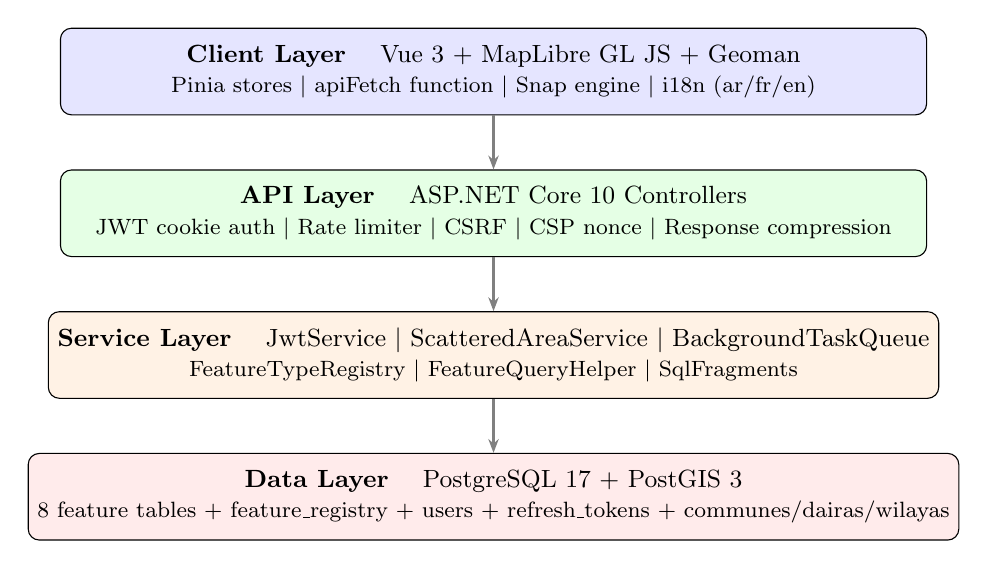
\begin{tikzpicture}[
  layer/.style={draw, rounded corners=4pt, minimum width=11cm,
                minimum height=1.1cm, align=center, font=\small},
  arr/.style={-{Stealth[length=5pt]}, thick, gray}
]
\node[layer, fill=blue!10]   (client)  at (0,0)   {%
  \textbf{Client Layer} \quad Vue 3 + MapLibre GL JS + Geoman \\
  {\footnotesize Pinia stores \textbar{} apiFetch function \textbar{} Snap engine \textbar{} i18n (ar/fr/en)}};

\node[layer, fill=green!10]  (api)     at (0,-1.8) {%
  \textbf{API Layer} \quad ASP.NET Core 10 Controllers \\
  {\footnotesize JWT cookie auth \textbar{} Rate limiter \textbar{} CSRF \textbar{} CSP nonce \textbar{} Response compression}};

\node[layer, fill=orange!10] (service) at (0,-3.6) {%
  \textbf{Service Layer} \quad JwtService \textbar{} ScatteredAreaService \textbar{} BackgroundTaskQueue \\
  {\footnotesize FeatureTypeRegistry \textbar{} FeatureQueryHelper \textbar{} SqlFragments}};

\node[layer, fill=red!8]     (db)      at (0,-5.4) {%
  \textbf{Data Layer} \quad PostgreSQL 17 + PostGIS 3 \\
  {\footnotesize 8 feature tables + feature\_registry + users + refresh\_tokens + communes/dairas/wilayas}};

\draw[arr] (client)  -- (api);
\draw[arr] (api)     -- (service);
\draw[arr] (service) -- (db);
\end{tikzpicture}
\caption{Four-layer architecture of NARS.}
\label{fig:architecture}
\end{figure}

\subsection{Technology Stack}

\begin{table}[H]
\centering
\caption{Technology stack summary}
\label{tab:stack}
\begin{tabular}{lll}
\toprule
\textbf{Component} & \textbf{Technology} & \textbf{Version} \\
\midrule
Backend runtime        & .NET (ASP.NET Core)          & 10.0 \\
ORM / query            & Entity Framework Core + ADO.NET & 10.x \\
Database               & PostgreSQL + PostGIS          & 17 / 3.x \\
Password hashing       & BCrypt.Net-Next               & --- \\
JWT library            & System.IdentityModel.Tokens.Jwt & --- \\
Frontend framework     & Vue 3 (Composition API)       & 3.5.x \\
State management       & Pinia                         & 3.x \\
Map engine             & MapLibre GL JS                & 5.x \\
Draw/edit layer        & Geoman for MapLibre (free)    & 0.8.x \\
Spatial utilities      & Turf.js                       & 7.x \\
Build tool             & Vite + vue-tsc                & 8.x / 3.x \\
XSS sanitiser          & DOMPurify                     & 3.x \\
Internationalisation   & vue-i18n                      & 11.x \\
\bottomrule
\end{tabular}
\end{table}

% ══════════════════════════════════════════════════════════════════════════════
\section{Data Flow: Feature Save Transaction}
\label{sec:save_transaction}

The save of a new feature involves a two-phase database transaction to
maintain the registry invariant (\cref{eq:registry_invariant}).

\begin{algorithm}[H]
\caption{SaveFeature transactional protocol}
\label{alg:save}
\begin{algorithmic}[1]
\Require type $\tau$, layer $\ell$, label $L$, data $D$, user $u$, commune $c$
\Ensure registry invariant (\ref{eq:registry_invariant}) holds after commit
\State Validate $\tau \in \mathcal{T}$ and $(\tau, \ell)$ is a valid type--layer pair
\State Validate $\tau \neq \texttt{area.scattered}$ \Comment{auto-computed only}
\State Validate $\abs{D_{\text{raw}}} \leq C_{\text{payload}}$ \Comment{eq.~\ref{eq:payload_bound}}
\If{$\tau = \texttt{house\_entrance}$ and $\ell = \texttt{main\_entrance}$}
  \State Extract $\texttt{roadDbId}$ from $D$; verify road exists and belongs to $u$
\EndIf
\State $\mathit{id} \leftarrow \texttt{Guid.CreateVersion7()}$ \Comment{UUID v7: monotonically sortable}
\State $e \leftarrow \texttt{FeatureTypeRegistry.CreateEntity}(\tau, \mathit{id}, u, \ell, L, D)$
\State \textbf{BEGIN} transaction $T$
\State Insert $e$ into the appropriate type table
\State Insert $(\mathit{id}, \tau)$ into \texttt{feature\_registry}
\State \textbf{COMMIT} $T$
\If{$\tau = \texttt{area}$}
  \State Enqueue scattered-area background refresh
\EndIf
\State \Return $\mathit{id}$
\end{algorithmic}
\end{algorithm}

The use of UUID v7 (time-ordered) as the primary key ensures that
the default \texttt{ORDER BY created\_at} in the load query is equivalent
to \texttt{ORDER BY id}, allowing future index optimisation.

% ══════════════════════════════════════════════════════════════════════════════
\section{Internationalisation Model}
\label{sec:i18n}

NARS supports three locales: English (\texttt{en}), French (\texttt{fr}),
and Arabic (\texttt{ar}). The locale catalogue is a JSON dictionary
$\mathcal{L}: \texttt{Key} \to \texttt{String}$ loaded by \texttt{vue-i18n}.
Arabic activates right-to-left layout via a CSS \texttt{dir="rtl"} attribute.

Administrative names are stored bilingual in the database
(\texttt{commune\_fr}/\texttt{commune\_ar},
\texttt{wilaya\_fr}/\texttt{wilaya\_ar}, etc.) and the API returns both
variants in every response, letting the client select the appropriate
column without an additional round-trip.

% ══════════════════════════════════════════════════════════════════════════════
\section{Circle Ring: Spherical Direct Problem}
\label{sec:circle_ring_correct}

The na\"ive formula in \cref{eq:circle_vertex} approximates the vertex
longitude offset with a flat-Earth cosine scale. The production implementation
in \texttt{geometry.ts} solves the exact \emph{spherical direct problem}:
given centre $(\varphi_c, \lambda_c)$, angular distance
$\alpha = r / R$, and bearing $\beta_k = 2\pi k / n$, the $k$-th vertex is:

\begin{align}
  \varphi_k &= \arcsin\!\bigl(
      \sin\varphi_c \cos\alpha
    + \cos\varphi_c \sin\alpha \cos\beta_k
  \bigr)
  \label{eq:sphere_direct_lat}\\[4pt]
  \lambda_k &= \lambda_c + \arctan2\!\Bigl(
      \sin\beta_k \sin\alpha \cos\varphi_c,\;
      \cos\alpha - \sin\varphi_c \sin\varphi_k
  \Bigr)
  \label{eq:sphere_direct_lng}
\end{align}

where all angles are in radians and coordinates are converted back to
degrees after computation. This is equivalent to Vincenty's direct formula
on a sphere and introduces no first-order approximation error in the
latitude direction. The na\"ive formula \eqref{eq:circle_vertex} is retained
in the documentation for pedagogical clarity; \eqref{eq:sphere_direct_lat}--\eqref{eq:sphere_direct_lng}
are what actually execute.

% ══════════════════════════════════════════════════════════════════════════════
\section{Road Direction Algorithm}
\label{sec:road_direction}

Road direction (start $\to$ end orientation) is required for rendering
directional arrows and for correctly sequencing house-entrance numbers
(\cref{sec:house_numbering}). The algorithm in
\texttt{road-directions.ts} runs in five phases.

\subsection{Phase 1 — Topology Graph Construction}

Let $\mathcal{R} = \{R_1, \ldots, R_n\}$ be the set of road polylines.
Each road $R_i$ is an ordered list of coordinates
$R_i = (p_0^{(i)}, \ldots, p_{m_i-1}^{(i)})$.
Define the \emph{junction threshold} $\delta_J = 30\ \mathrm{m}$.

For every ordered pair $(R_i, R_j)$ with $i \neq j$, two junction types are detected:

\paragraph{T-junction.}
An endpoint $p \in \{p_0^{(j)}, p_{m_j-1}^{(j)}\}$ that satisfies
\[
  d_{\text{geo}}(p, p_0^{(i)}) > \delta_J
  \quad\text{and}\quad
  d_{\text{geo}}(p, p_{m_i-1}^{(i)}) > \delta_J
\]
yet whose nearest point
on the body of $R_i$ is within $\delta_J$:
\begin{equation}
  q^* = \proj_{R_i}(p), \quad d_{\text{geo}}(p, q^*) \leq \delta_J
  \label{eq:t_junction}
\end{equation}

\paragraph{X-junction.}
Any geometric intersection point of lines $R_i$ and $R_j$ that lies strictly
in the interior of both (not within $\delta_J$ of either road's endpoints).

The junctions on $R_i$ are sorted by arc-length parameter, deduplicated
(any two within $\delta_J$ are merged), and used to split $R_i$ into
sub-segments $S_{i,1}, \ldots, S_{i,k_i}$. Each sub-segment becomes an
undirected edge in the topology graph $G = (V, E)$, where vertices are
shared at all junction points (merged within $\delta_J$).

\begin{definition}[Topology graph]
$G = (V, E)$ where
\begin{equation*}
  V = \{v \in \mathcal{G} \mid v \text{ is an endpoint or junction point}\}
\end{equation*}
and $e = (v_a, v_b, s) \in E$ iff sub-segment $s$ connects $v_a$ to $v_b$.
Nodes within $\delta_J$ of each other are unified.
\end{definition}

\subsection{Phase 2A — City-Centre Orientation (DFS)}

When at least one city centre exists, a depth-first search from the
city-centre perimeter assigns orientation to every reachable segment.

Let $\mathcal{C} = (c, r)$ be a city centre (centre $c$, radius $r$).
The \emph{seed nodes} are:
\begin{equation}
  V_{\text{seed}} = \left\{ v \in V \;\middle|\;
    \abs{d_{\text{geo}}(c, v) - r} \leq \delta_J
  \right\}
  \label{eq:seed_nodes}
\end{equation}

For each seed $v_s \in V_{\text{seed}}$, \textsc{OrientFrom}$(v_s)$ is called.
At each recursive call with \textit{fromNode} $v_f$:
\begin{enumerate}
  \item Collect unvisited, unassigned edges incident to $v_f$, sorted by
    ascending distance of their far endpoint to $c$
    (closest roads oriented first).
  \item For each edge $e = (v_f, v_{\text{to}}, s)$:
    \begin{equation}
      s.\mathrm{reversed} = \left[
        d_{\text{geo}}(s_0, v_f) > d_{\text{geo}}(s_{|\cdot|-1}, v_f)
      \right]
      \label{eq:segment_orient}
    \end{equation}
    where $s_0$ and $s_{|s|-1}$ are the first and last coordinates of $s$.
  \item Mark $e$ and all segments of the same road as visited.
  \item Recurse: \textsc{OrientFrom}$(v_{\text{to}})$.
\end{enumerate}

\subsection{Phase 2B — Geographic Fallback}

For roads unreached by the DFS (or when no city centre exists), orientation
is assigned by cardinal direction:
\begin{equation}
  s.\mathrm{reversed} =
  \begin{cases}
    \varphi_0 < \varphi_{|\cdot|-1} & \text{if } |\Delta\varphi| \geq |\Delta\lambda| \quad
      \text{(N--S road: start at north)} \\
    \lambda_0 < \lambda_{|\cdot|-1} & \text{otherwise} \quad
      \text{(E--W road: start at east)}
  \end{cases}
  \label{eq:geographic_fallback}
\end{equation}

\subsection{Phase 3 — Majority Vote}

Sub-segments of the same road may have received different orientations via
different DFS paths. The final orientation of road $R_i$ is determined by
majority vote over its $k_i$ sub-segments:

\begin{equation}
  R_i.\mathrm{reversed} =
  \left[
    \sum_{j=1}^{k_i} \mathbf{1}[S_{i,j}.\mathrm{reversed}]
    > \frac{k_i}{2}
  \right]
  \label{eq:majority_vote}
\end{equation}

\subsection{Phase 4 — Dead-End Correction}

Let $\deg(v)$ be the degree of node $v$ in $G$. If a road's first endpoint
$v_a$ has $\deg(v_a) = 1$ and its last endpoint $v_b$ has $\deg(v_b) > 1$,
the connected side ($v_b$) must be the \emph{from} side, overriding the
majority vote:

\begin{equation}
  R_i.\mathrm{reversed} = \neg\,[\deg(v_a) > \deg(v_b)]
  \label{eq:dead_end}
\end{equation}

When both endpoints have $\deg = 1$ (road split by a T-junction on its
body), the from-side is the endpoint closer to the city centre.

\subsection{Segment Bearing}

The directional arrow angle $\theta$ for endpoint markers is computed in
MapLibre screen space:
\begin{equation}
  \theta = \arctan2\!\left(
    \Pi(p_{i+1})_y - \Pi(p_i)_y,\;
    \Pi(p_{i+1})_x - \Pi(p_i)_x
  \right) \cdot \frac{180}{\pi}
  \label{eq:bearing}
\end{equation}

where $\Pi$ is the MapLibre \texttt{project} function at the current zoom level.

% ══════════════════════════════════════════════════════════════════════════════
\section{House Entrance Numbering}
\label{sec:house_numbering}

House entrances connected to a reference road are assigned numbers by
projecting each unassigned entrance onto the road's polyline, sorting
by arc-length, and allocating odd numbers to the left side and even
numbers to the right side.

\subsection{Arc-Length Projection}

For a road $R = (p_0, \ldots, p_{m-1})$ (as a Turf.js \texttt{LineString})
and an entrance point $e$, the \emph{arc-length parameter}
$\ell(e) \geq 0$ is the cumulative metric distance from $p_0$ to the
nearest point on $R$:

\begin{equation}
  e^* = \operatorname{NearestPointOnLine}(R, e), \quad
  \ell(e) = \texttt{snapped.properties.location}
  \label{eq:arc_length}
\end{equation}

computed by Turf.js \texttt{nearestPointOnLine} with \texttt{units="meters"}.

\subsection{Numbering Assignment}

Let $\mathcal{E}_u$ be the set of unassigned entrances projected and sorted
by arc-length: $e_1, e_2, \ldots, e_k$ with
$\ell(e_1) \leq \ell(e_2) \leq \cdots \leq \ell(e_k)$.

The seed counters are initialised from already-assigned entrances on the
same road:
\begin{align}
  o_0 &= \max\!\left(\{n \mid n \text{ odd},\;
    n \text{ assigned to a left entrance on } R\} \cup \{-1\}\right) + 2
  \label{eq:odd_seed} \\
  e_0 &= \max\!\left(\{n \mid n \text{ even},\;
    n \text{ assigned to a right entrance on } R\} \cup \{0\}\right) + 2
  \label{eq:even_seed}
\end{align}

The number assigned to the $i$-th unassigned entrance is:
\begin{equation}
  N(e_i) =
  \begin{cases}
    o_j \leftarrow o_{j-1} + 2 & \text{if } e_i.\mathrm{side} = \mathrm{left}  \\
    e_j \leftarrow e_{j-1} + 2 & \text{if } e_i.\mathrm{side} = \mathrm{right}
  \end{cases}
  \label{eq:entrance_number}
\end{equation}

where $j$ increments independently for odd and even counters, ensuring
no two left-side (or right-side) entrances share a number.

This scheme is consistent with the international convention of odd numbers
on one side of a street and even on the other, sequenced in order of
increasing distance from the origin of the road.

% ══════════════════════════════════════════════════════════════════════════════
\section{Point-in-Polygon: Ray-Casting Algorithm}
\label{sec:pip}

Two spatial hit-tests use a client-side even-odd rule rather than a
PostGIS query: (1) checking whether a new feature falls within the
municipality boundary, and (2) checking whether a point lies in the
scattered area. Both use the same \texttt{pointInRing} function from
\texttt{geometry.ts}.

\begin{definition}[Even-odd rule]
A point $q = (\varphi, \lambda)$ lies \emph{inside} polygon ring
$\mathcal{P} = (v_0, v_1, \ldots, v_{n-1})$ (with $v_n = v_0$) if and
only if the number of ring edges that cross the horizontal ray emanating
rightward from $q$ is odd:

\begin{equation}
  \mathbf{1}[q \in \mathcal{P}] =
  \left(\sum_{i=0}^{n-1} \mathbf{1}[\text{edge } (v_i, v_{i+1})
  \text{ crosses the ray}]\right) \bmod 2 = 1
  \label{eq:pip_even_odd}
\end{equation}
\end{definition}

An edge $(v_i, v_{i+1})$ with $v_i = (\varphi_i, \lambda_i)$
crosses the horizontal ray from $(\varphi, \lambda)$ when:

\begin{equation}
  \bigl[(\lambda_i > \lambda) \neq (\lambda_{i+1} > \lambda)\bigr]
  \;\land\;
  \left[
    \varphi < \frac{(\varphi_{i+1} - \varphi_i)(\lambda - \lambda_i)}
                   {\lambda_{i+1} - \lambda_i} + \varphi_i
  \right]
  \label{eq:pip_crossing}
\end{equation}

The implementation toggles an \texttt{inside} boolean for each crossing,
producing $O(n)$ time and $O(1)$ space complexity.

For the scattered area (\cref{sec:scattered}), which may contain holes,
the predicate is extended:

\begin{equation}
  q \in S \iff
  \text{pointInRing}(q, S.\mathrm{outer})
  \;\land\;
  \forall\, H \in S.\mathrm{holes}:\;
  \neg\,\text{pointInRing}(q, H)
  \label{eq:pip_with_holes}
\end{equation}

% ══════════════════════════════════════════════════════════════════════════════
\section{Undo Stack}
\label{sec:undo}

NARS implements a \emph{delete-only} undo model: the undo stack captures
deleted features; vertex-level undo during drawing is delegated to Geoman's
built-in right-click remove.

\begin{definition}[Undo stack]
The undo stack $\mathcal{U}$ is a last-in first-out sequence of records:
\begin{equation}
  \mathcal{U} = \langle (e_1, k_1), (e_2, k_2), \ldots, (e_m, k_m) \rangle
  \label{eq:undo_stack}
\end{equation}
where $e_i \in \texttt{LayerEntry}$ is the deleted feature's in-memory
representation and $k_i \in \texttt{Phase}$ is its phase key.
\end{definition}

\subsection{Record}

Before a delete request is dispatched to the API, the entry is pushed:
\begin{equation}
  \mathcal{U} \leftarrow \mathcal{U} \cdot \langle (e, k) \rangle
  \label{eq:undo_push}
\end{equation}

\subsection{Restore}

On Ctrl+Z, the stack is popped and the entry is re-saved via
\texttt{POST /api/features}. This allocates a \emph{new} UUID for the
restored feature:

\begin{equation}
  \text{id}_{\text{new}} \neq \text{id}_{\text{old}}
  \label{eq:undo_new_id}
\end{equation}

This has an important cross-reference consequence: any
\texttt{secondary\_entrance} records that referenced the old main-entrance
ID via \texttt{mainEntranceDbId} must be updated. The restore procedure
performs this repair in-memory:

\begin{equation}
  \begin{aligned}
    \forall e' \in \texttt{houseEntrances}:&\;
    e'.\texttt{mainEntranceDbId} = \text{id}_{\text{old}} \\
    &\quad\implies\;
    e'.\texttt{mainEntranceDbId} \leftarrow \text{id}_{\text{new}}
  \end{aligned}
  \label{eq:undo_ref_repair}
\end{equation}

\begin{remark}
The undo stack lives only in browser memory and is cleared on page reload.
It provides a best-effort safety net for accidental deletions within a
single session, not a durable audit trail.
\end{remark}

% ══════════════════════════════════════════════════════════════════════════════
\section{Client-Side Validation Pipeline}
\label{sec:client_validation}

Before dispatching to the server, the frontend performs two lightweight
checks that catch the most common user errors without a network round-trip.

\subsection{Geometry Cardinality}

A feature is rejected on the client if its coordinate sequence is too
short to define the requested geometry (checked in
\texttt{draw-save.ts::validateGeometry}):

\begin{equation}
  \texttt{LineString}: \ m \geq 2, \qquad
  \texttt{Polygon}: \ m \geq 3
  \label{eq:min_cardinality}
\end{equation}

where $m$ is the coordinate count. This mirrors MapLibre Geoman's own
minimum-vertex constraints, preventing malformed geometries from reaching
the server.

\subsection{City-Centre Radius Bounds}

City-centre features are stored as circles; the client rejects any radius
outside the configured bounds (\texttt{draw-save.ts::validateGeometry}):

\begin{equation}
  r_{\min} \leq r \leq r_{\max}, \qquad
  r_{\min} = 5\ \mathrm{m}, \quad r_{\max} = 50{,}000\ \mathrm{m}
  \label{eq:city_radius_bounds}
\end{equation}

When a city centre is drawn as a polygon, the radius is derived from the
circumradius of the drawn ring before this check is applied.

\subsection{Two-Stage Validation Architecture}

\Cref{fig:validation_flow} summarises the overall two-stage structure:
client-side fast checks followed by server-side PostGIS spatial predicates.

\begin{figure}[H]
\centering
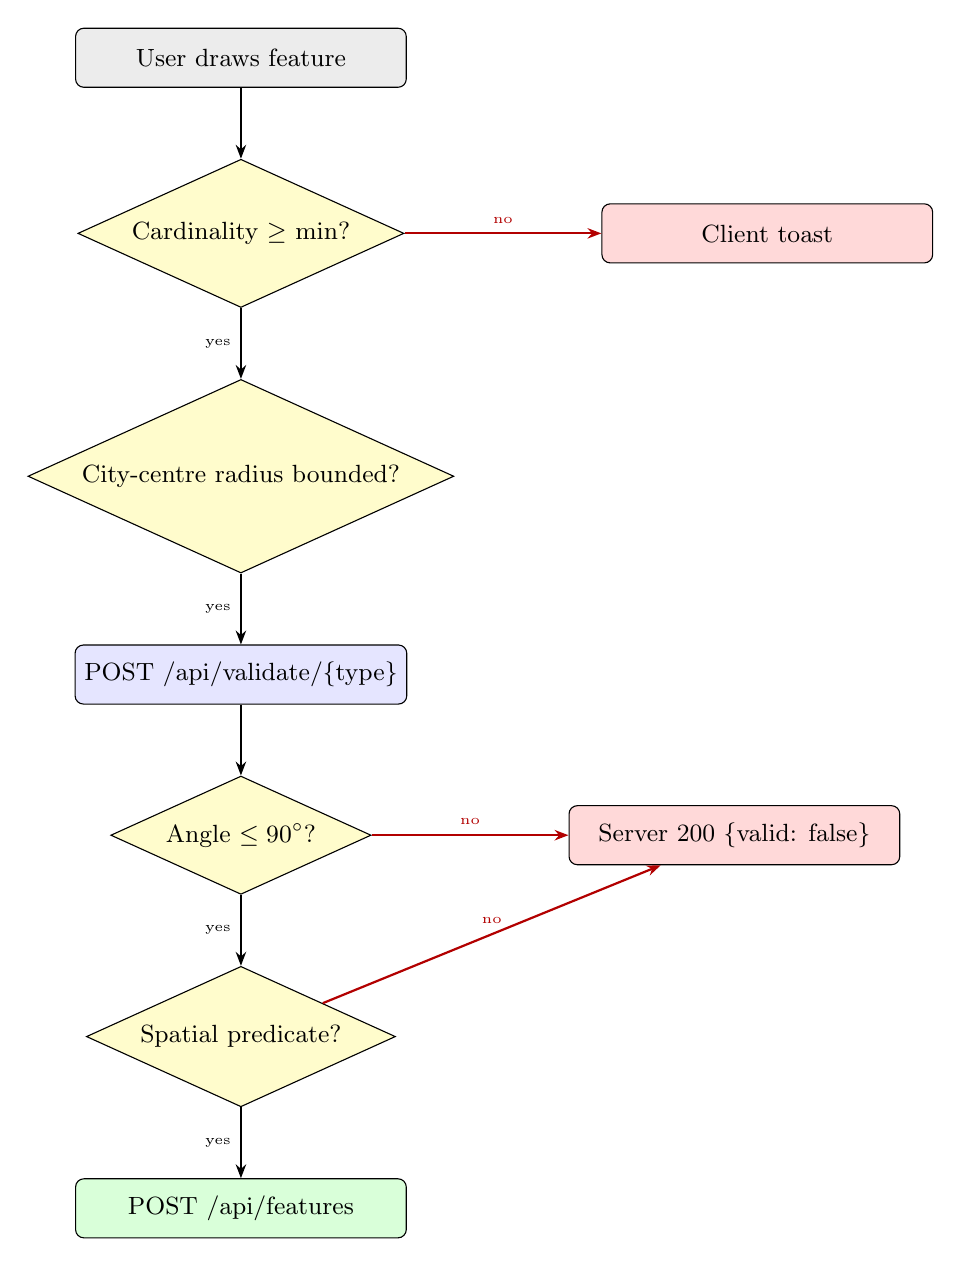
\begin{tikzpicture}[
  node distance=0.9cm,
  box/.style={draw, rounded corners=3pt, minimum width=4.2cm,
              minimum height=0.75cm, align=center, font=\small},
  dec/.style={draw, diamond, minimum width=3cm, minimum height=0.7cm,
              align=center, font=\small, aspect=2.2},
  arr/.style={-{Stealth[length=5pt]}, thick},
  rej/.style={-{Stealth[length=5pt]}, thick, red!70!black}
]
\node[box, fill=gray!15] (input)  {User draws feature};
\node[dec, fill=yellow!20, below=of input] (c1) {Cardinality $\geq$ min?};
\node[dec, fill=yellow!20, below=of c1] (c2) {City-centre radius bounded?};
\node[box, fill=blue!10, below=of c2] (api) {POST /api/validate/\{type\}};
\node[dec, fill=yellow!20, below=of api] (s1) {Angle $\leq 90^{\circ}$?};
\node[dec, fill=yellow!20, below=of s1] (s2) {Spatial predicate?};
\node[box, fill=green!15, below=of s2] (save) {POST /api/features};
\node[box, fill=red!15, right=2.5cm of c1] (rej1) {Client toast};
\node[box, fill=red!15, right=2.5cm of s1] (rej2) {Server 200 \{valid: false\}};

\draw[arr] (input) -- (c1);
\draw[arr] (c1) -- node[left, font=\tiny]{yes} (c2);
\draw[rej] (c1) -- node[above, font=\tiny]{no} (rej1);
\draw[arr] (c2) -- node[left, font=\tiny]{yes} (api);
\draw[arr] (api) -- (s1);
\draw[arr] (s1) -- node[left, font=\tiny]{yes} (s2);
\draw[rej] (s1) -- node[above, font=\tiny]{no} (rej2);
\draw[arr] (s2) -- node[left, font=\tiny]{yes} (save);
\draw[rej] (s2) -- node[above, font=\tiny]{no} (rej2);
\end{tikzpicture}
\caption{Two-stage validation flow for feature saves.
Client-side checks (yellow) prevent trivial invalid inputs without a
network round-trip. Server-side PostGIS checks enforce spatial correctness.}
\label{fig:validation_flow}
\end{figure}

% ══════════════════════════════════════════════════════════════════════════════
\section{Database Schema}
\label{sec:schema}

\subsection{Relation Definitions}

The database comprises 18 tables. \Cref{tab:schema} summarises the
primary keys, foreign keys, and key index definitions as derived from
\texttt{AppDbContext.cs} and the EF Core model configuration.

\begin{table}[H]
\centering
\caption{Database schema summary}
\label{tab:schema}
\begin{tabularx}{\textwidth}{llXX}
\toprule
\textbf{Table} & \textbf{PK} & \textbf{FK} & \textbf{Notable indices / constraints} \\
\midrule
\texttt{users}
  & \texttt{id} (UUID v7)
  &
  & UNIQUE(\texttt{email}), UNIQUE(\texttt{username}) \\
\texttt{refresh\_\allowbreak{}tokens}
  & \texttt{id} (UUID)
  & \texttt{user\_\allowbreak{}id} $\to$ \texttt{users}
  & \texttt{ix\_\allowbreak{}refresh\_\allowbreak{}tokens\_\allowbreak{}token\_\allowbreak{}hash} \\
\texttt{wilayas}
  & \texttt{wilaya\_\allowbreak{}id} (int)
  &
  & Static reference table \\
\texttt{dairas}
  & \texttt{daira\_\allowbreak{}id} (int)
  & \texttt{wilaya\_\allowbreak{}id} $\to$ \texttt{wilayas}
  & \texttt{ix\_\allowbreak{}dairas\_\allowbreak{}wilaya\_\allowbreak{}id} \\
\texttt{communes}
  & \texttt{commune\_\allowbreak{}id} (int)
  & \texttt{daira\_\allowbreak{}id} $\to$ \texttt{dairas}
  & \texttt{ix\_\allowbreak{}communes\_\allowbreak{}daira\_\allowbreak{}id} \\
\texttt{communes\_\allowbreak{}boundaries}
  & \texttt{commune\_\allowbreak{}id} (int)
  &
  & GIST index on \texttt{geometry} \\
\texttt{feature\_\allowbreak{}registry}
  & \texttt{id} (UUID v7)
  &
  & \texttt{feature\_\allowbreak{}type} string \\
\texttt{areas}
  & \texttt{id} (UUID v7)
  &
  & \texttt{ix\_\allowbreak{}areas\_\allowbreak{}user\_\allowbreak{}id}, \texttt{ix\_\allowbreak{}areas\_\allowbreak{}user\_\allowbreak{}layer} \\
\texttt{districts}
  & \texttt{id} (UUID v7)
  &
  & \texttt{ix\_\allowbreak{}districts\_\allowbreak{}user\_\allowbreak{}id} \\
\texttt{city\_\allowbreak{}centers}
  & \texttt{id} (UUID v7)
  &
  & \texttt{ix\_\allowbreak{}city\_\allowbreak{}centers\_\allowbreak{}user\_\allowbreak{}id} \\
\texttt{roads}
  & \texttt{id} (UUID v7)
  &
  & \texttt{ix\_\allowbreak{}roads\_\allowbreak{}user\_\allowbreak{}id}, \texttt{ix\_\allowbreak{}roads\_\allowbreak{}user\_\allowbreak{}layer} \\
\texttt{house\_\allowbreak{}entrances}
  & \texttt{id} (UUID v7)
  & \texttt{road\_\allowbreak{}id} $\to$ \texttt{roads} (nullable)
  & \texttt{ix\_\allowbreak{}house\_\allowbreak{}entrances\_\allowbreak{}road\_\allowbreak{}id} (partial, \texttt{road\_\allowbreak{}id IS NOT NULL}) \\
\texttt{public\_\allowbreak{}buildings}
  & \texttt{id} (UUID v7)
  &
  & \texttt{ix\_\allowbreak{}public\_\allowbreak{}buildings\_\allowbreak{}user\_\allowbreak{}id} \\
\texttt{public\_\allowbreak{}spaces}
  & \texttt{id} (UUID v7)
  &
  & \texttt{ix\_\allowbreak{}public\_\allowbreak{}spaces\_\allowbreak{}user\_\allowbreak{}id} \\
\texttt{naming\_\allowbreak{}panels}
  & \texttt{id} (UUID v7)
  &
  & \texttt{ix\_\allowbreak{}naming\_\allowbreak{}panels\_\allowbreak{}user\_\allowbreak{}id} \\
\texttt{error\_\allowbreak{}logs}
  & \texttt{id} (UUID v7)
  & \texttt{user\_\allowbreak{}id} $\to$ \texttt{users} (nullable)
  & \texttt{ix\_\allowbreak{}error\_\allowbreak{}logs\_\allowbreak{}user\_\allowbreak{}id}, \texttt{ix\_\allowbreak{}error\_\allowbreak{}logs\_\allowbreak{}level}, \texttt{ix\_\allowbreak{}error\_\allowbreak{}logs\_\allowbreak{}created\_\allowbreak{}at} \\
\texttt{inspections}
  & \texttt{id} (UUID v7)
  & \texttt{user\_\allowbreak{}id} $\to$ \texttt{users}
  & \texttt{ix\_\allowbreak{}inspections\_\allowbreak{}user\_\allowbreak{}id}, \texttt{ix\_\allowbreak{}inspections\_\allowbreak{}feature\_\allowbreak{}created} \\
\texttt{ai\_\allowbreak{}draft\_\allowbreak{}features}
  & \texttt{id} (UUID v7)
  & \texttt{commune\_\allowbreak{}id} $\to$ \texttt{communes}, \texttt{reviewed\_\allowbreak{}by} $\to$ \texttt{users} (nullable)
  & \texttt{ix\_\allowbreak{}ai\_\allowbreak{}draft\_\allowbreak{}status}, \texttt{ix\_\allowbreak{}ai\_\allowbreak{}draft\_\allowbreak{}created\_\allowbreak{}at} \\
\bottomrule
\end{tabularx}
\end{table}

\subsection{Feature Base Schema}

All eight feature tables share the same base schema
(from \texttt{FeatureBase.cs}):

\begin{equation}
  \texttt{feature} = (\underbrace{\texttt{id}}_{\text{UUID v7}},\;
  \texttt{user\_id},\; \texttt{label},\;
  \underbrace{\texttt{data}}_{\text{JSON text}},\;
  \texttt{layer},\; \texttt{created\_at},\; \texttt{updated\_at})
  \label{eq:feature_base}
\end{equation}

Geometry is \emph{not} stored in a native PostGIS column; it is embedded as
a JSON array of $\{\texttt{lat}, \texttt{lng}\}$ objects within \texttt{data}.
This design prioritises schema flexibility over spatial index coverage.
All PostGIS predicates reconstruct geometry from the JSON at query time via the
\texttt{SqlFragments.PolygonFromData} and \texttt{LineStringFromData} fragments.

\subsection{UUID v7 Temporal Ordering}

Primary keys are generated client-side using \texttt{Guid.CreateVersion7()},
which encodes a Unix millisecond timestamp in the high 48 bits of the UUID:

\begin{equation}
  \begin{aligned}
    \text{UUID v7} &=
      \underbrace{\text{48 bits: ms timestamp}}_{\text{monotonic}}
      \;\|\;
      \underbrace{\text{4 bits: version = 7}}_{} \\
    &\quad\|\;
      \underbrace{\text{12 bits: seq counter}}_{\text{sub-ms ordering}}
      \;\|\;
      \underbrace{\text{2 bits: variant}}_{} \\
    &\quad\|\;
      \underbrace{\text{62 bits: random}}_{\text{uniqueness}}
  \end{aligned}
  \label{eq:uuid_v7}
\end{equation}

This ensures that the default \texttt{ORDER BY created\_at} and
\texttt{ORDER BY id} produce identical orderings, enabling future migration
from timestamp-based to UUID-based ordering with no query changes.

% ══════════════════════════════════════════════════════════════════════════════
\section{Conclusions}
\label{sec:conclusions}

This document has presented a complete mathematical specification of the
National Addressing Reference System. The key formal results are:

\begin{enumerate}
  \item The road angular-deviation bound (\cref{eq:road_angle_predicate})
    guarantees that no road segment subtends an obtuse deflection angle,
    which is a necessary condition for unambiguous address assignment.

  \item The district non-overlap (\cref{eq:district_no_overlap}),
    adjacency (\cref{eq:district_adjacency}), and coverage
    (\cref{eq:coverage}) conditions collectively ensure that the district
    partition is a topological valid tiling of the urban areas up to a
    $10\ \mathrm{m}$ tolerance.

  \item The refresh-token rotation protocol (\cref{sec:refresh}) provides
    single-use guarantees for refresh tokens through row-level locking,
    preventing concurrent reuse without introducing distributed
    coordination.

  \item The sliding-window rate limiter (\cref{eq:sliding_window}) bounds
    the per-IP request rate, and the account-lockout mechanism
    (\cref{eq:lockout}) provides a secondary defence against
    credential-stuffing attacks.

  \item The road-direction algorithm (\cref{sec:road_direction}) constructs
    a full topology graph handling T-junctions and X-junctions in
    $O(n^2)$ time, then orients every segment via a depth-first search
    from the city-centre perimeter, with geographic fallback for isolated
    roads.

  \item The house-entrance numbering scheme (\cref{sec:house_numbering})
    is well-defined and consistent: arc-length projection combined with
    odd/even side assignment guarantees that no two entrances on the
    same side of a road share a number, and the seeding from already-assigned
    numbers prevents gaps in the sequence.

  \item The circle ring computation (\cref{sec:circle_ring_correct}) solves
    the spherical direct problem exactly, producing correct vertex positions
    at all latitudes without the cosine-scale approximation error of the
    na\"ive formula.

  \item The even-odd ray-casting algorithm (\cref{sec:pip}) provides
    $O(n)$ point-in-polygon classification for both the municipality
    boundary and scattered area polygons, without any server round-trip.
\end{enumerate}

Future work should consider migrating coordinate storage from JSON arrays
to native PostGIS geometry columns, which would eliminate the
coordinate-order swap in \texttt{SqlFragments.cs}, enable spatial
indexing on feature geometries (currently only possible via
\texttt{ST\_GeomFromGeoJSON} at query time), and reduce storage overhead
by approximately $40\,\%$.

% ══════════════════════════════════════════════════════════════════════════════
\section*{Acknowledgements}

The authors acknowledge the use of the following open-source projects:
PostgreSQL, PostGIS, ASP.NET Core, Entity Framework Core, Vue 3, MapLibre
GL JS, Geoman, Turf.js, DOMPurify, and vue-i18n.

% ══════════════════════════════════════════════════════════════════════════════
\begin{thebibliography}{99}

\bibitem{wgs84}
National Geospatial-Intelligence Agency (2014)
Department of Defense World Geodetic System 1984: Its Definition and
Relationships with Local Geodetic Systems, 4th edn.
NGA.STND.0036\_1.0.0\_WGS84, Springfield

\bibitem{haversine}
Sinnott RW (1984) Virtues of the Haversine.
Sky and Telescope 68(2):159

\bibitem{bcrypt}
Provos N, Mazières D (1999) A Future-Adaptable Password Scheme.
In: Proc USENIX Annual Technical Conference, FREENIX Track, Monterey, 81--91

\bibitem{jwt_rfc}
Jones M, Bradley J, Sakimura N (2015) JSON Web Token (JWT).
RFC 7519. Internet Engineering Task Force.
\url{https://doi.org/10.17487/RFC7519}

\bibitem{postgis}
Obe R, Hsu L (2021) PostGIS in Action, 3rd edn.
Manning, Shelter Island

\bibitem{hmac_rfc}
Krawczyk H, Bellare M, Canetti R (1997) HMAC: Keyed-Hashing for Message
Authentication. RFC 2104. Internet Engineering Task Force.
\url{https://doi.org/10.17487/RFC2104}

\bibitem{maplibre}
MapLibre Contributors (2024) MapLibre GL JS.
\url{https://maplibre.org}. Accessed 18 April 2026

\bibitem{geojson_rfc}
Butler H, Daly M, Doyle A, Gillies S, Hagen S, Schaub T (2016)
The GeoJSON Format. RFC 7946. Internet Engineering Task Force.
\url{https://doi.org/10.17487/RFC7946}

\bibitem{owasp_csrf}
OWASP Foundation (2023) Cross-Site Request Forgery (CSRF) Prevention
Cheat Sheet. \url{https://cheatsheetseries.owasp.org/cheatsheets/Cross-Site\_Request\_Forgery\_Prevention\_Cheat\_Sheet.html}. Accessed 18 April 2026

\bibitem{sliding_window}
Leaky Bucket vs Token Bucket: Rate Limiting Algorithms (2022).
Microsoft Azure Architecture Center.
\url{https://learn.microsoft.com/en-us/azure/architecture/patterns/rate-limiting-pattern}.
Accessed 18 April 2026

\bibitem{uuid7}
Davis K, Peabody B, Leach P (2022) A New Format for Time-Ordered
Universally Unique Identifier (UUID). RFC 9562.
Internet Engineering Task Force.
\url{https://doi.org/10.17487/RFC9562}

\end{thebibliography}

\end{document}
